%---------------------------------------------------------------
\chapter{Reliable PUF response reconstruction}\label{sec:response_extraction} % TODO should this be its own section or part of the previous one?
%---------------------------------------------------------------

Since \gls{sram} \glspl{puf} are classified as weak (they do not have a large challenge-response pair set), their main use is for cryptographic key generation. The keys need to be extracted without error, otherwise the cryptographic algorithms that use the keys will not work. Therefore, methods of reliable response reconstruction are used to stabilize the \gls{puf} response.

In this chapter, stable bit preselection and \gls{ecc} techniques are used on top of the designed memory power-control methods in order to stabilize the response of the ESP32 \gls{sram} \gls{puf}. Then, a \gls{puf} design that combines the two power-control methods is presented. At the end, the enrollment process of key generation is discussed and the resulting \gls{sram} \gls{puf} based key generation is tested on all \glspl{mcu} at different operating temperatures. \gls{puf} design with only a single response will be implemented.

%--------------------------------
\section{Stable bit preselection}
%--------------------------------

Stable bit preselection consists of two steps. First, during the enrollment phase, the stable bits are selected and a stable bit mask is created. The mask is then saved to a non-volatile memory of the device. When a \gls{puf} response needs to be reconstructed, the mask is loaded and the unstable bits are discarded.

Direct bit preselection was used to obtain the stable bits. Other methods that try to preselect stable bits exist, such as the indirect preselection method described in Section~\ref{sec:indirect_bit_preselection}. However, the discussed stability test which measures the stabilization time of each memory cell, cannot be used for our \gls{puf} implementation. The deep sleep method of memory power-control does not enable turn off intervals of less than 1000 $\mu{}S$. Thus, it is not possible to carry out the test accurately.

\subsubsection*{Stable bit mask creation}

The stable bit mask is created by measuring a \gls{puf} response multiple times. An average startup value $\bar{x}$ of each bit is then calculated from the responses. Then, a threshold value, called the error rate $E_r$, needs to be selected. Bits with average value $\bar{x} \leq E_r$ (stable `0') or $\bar{x} \geq (1-E_r)$ (stable `1') are declared as stable.

Two techniques were used to generate the stable bit mask. First, 1000 measurements of the \gls{puf} response were taken in 20 °C and the mask was created using the above-described method.

The second technique was inspired by~\cite{Hanova2020}. Twelve different intermediate masks were created, each from 1000 measurements of the \gls{puf} response. The measurements for each mask were captured in different operating conditions.\footnote{The temperatures of -40, -30, -20, -10, 0, 10, 20, 30, 40, 50, 60 and 70~°C were used for the twelve masks.} Then, the final mask was calculated as a bitwise logical AND from the twelve intermediate masks---a bit is declared stable if it is stable at all twelve operating temperatures.

\subsubsection*{Results}

Table~\ref{table:stable_bits} shows the percentage of stable bits found in a 4 KB sample \gls{puf} response for all \glspl{mcu}. Three different error rates were chosen, 10~\%, 1~\% and 0.1~\%. As expected, lower error rate reduces the number of stable bits. Moreover, the temperature range mask (created by the second technique) further reduced the percentage of stable bits by about 17~\% compared to the 20~°C mask. Only the results for the deep sleep method of power-control are presented, as the temperature range mask cannot be used for the \gls{rtc} \gls{sram} method (because of the memory freezing effect). The error rate of 0.1~\% was chosen for the \gls{sram} \gls{puf} implementation as it provides the best reliability with only a minor reduction of available bits.

\begin{table}[ht!]
    \centering
    \begin{tabular}{c||ccc|ccc}
        \multicolumn{1}{c}{} & \multicolumn{3}{c}{\textbf{20 °C mask}} & \multicolumn{3}{c}{\textbf{Temperature range mask}} \\
    \toprule
    \textbf{MCU} &  \textbf{10 \%} &  \textbf{1.0 \%} &  \textbf{0.1 \%} &  \textbf{10 \%} &  \textbf{1.0 \%} &  \textbf{0.1 \%} \\
    \midrule
    1    &   87.37 &  77.32 &  71.24 &    72.39 &   62.87 &   56.43 \\
    2    &   87.56 &  77.66 &  71.58 &    72.79 &   63.05 &   56.67 \\
    3    &   87.94 &  78.60 &  72.82 &    73.54 &   64.29 &   58.24 \\
    4    &   87.55 &  77.50 &  71.34 &    72.31 &   62.90 &   56.76 \\
    5    &   87.75 &  77.91 &  71.82 &    74.41 &   64.91 &   58.47 \\
    6    &   87.89 &  78.09 &  72.11 &    73.18 &   63.72 &   57.80 \\
    7    &   88.11 &  78.97 &  72.93 &    73.93 &   64.56 &   58.34 \\
    8    &   87.58 &  77.89 &  72.04 &    73.93 &   64.59 &   58.52 \\
    9    &   88.03 &  78.49 &  72.38 &    74.12 &   64.55 &   58.25 \\
    10   &   87.70 &  77.88 &  71.83 &    73.43 &   63.84 &   57.54 \\
    11   &   89.07 &  80.03 &  74.57 &    75.36 &   66.24 &   60.24 \\
    12   &   87.56 &  77.60 &  71.51 &    72.64 &   62.93 &   56.76 \\
    13   &   88.22 &  79.13 &  73.32 &    73.89 &   65.01 &   59.09 \\
    14   &   87.50 &  77.67 &  71.80 &    73.04 &   63.68 &   57.60 \\
    15   &   87.30 &  77.18 &  71.51 &    72.42 &   62.95 &   56.71 \\
    16   &   88.00 &  78.59 &  72.84 &    70.15 &   61.36 &   55.54 \\
    \textbf{mean} &   87.82 &  78.16 &  72.23 &    73.22 &   63.84 &   57.68 \\
    \bottomrule
    \end{tabular}
    \captionsetup{justification=centering,margin=0.5cm}
    \caption{Percentage of stable bits across all MCUs. Three different error rates (10 \%, 1 \% and 0.1 \%) and two stable bit selection methods were used.}
    \label{table:stable_bits}
    \vspace{-1.5em}
\end{table}

Table~\ref{table:reliability_stable_bits} shows reliability of \gls{puf} responses at different operating temperatures and for all \glspl{mcu}. The reference response was obtained at 20 °C and only the stable bits of the responses were selected using the 20 °C mask. The table shows results using the deep sleep power-control method, but the \gls{rtc} \gls{sram} method shows nearly identical results above -10~°C.

The best reliability is observed at 20~°C, since this is the temperature the reference and stable bit mask were calculated at. With increasing distance from 20~°C, the reliability reduces. However, reliability was increased significantly thanks to the stable bit preselection. Reliability results without the preselection can be found in Table~\ref{table:reliability_deep_sleep}.

\begin{table}[ht!]
    \centering
    \begin{tabular}{c||rrrrrrrrrr}
    \toprule
    \textbf{MCU} & \textbf{-40°C} & \textbf{-30°C} & \textbf{-20°C} & \textbf{-10°C} & \textbf{0°C} & \textbf{10°C} & \textbf{20°C} & \textbf{30°C} & \textbf{50°C} & \textbf{70°C} \\
    \midrule
    1    &  98.27 &  98.96 &  99.45 &  99.75 & 99.88 & 99.92 & 99.99 & 99.97 & 99.83 & 99.42 \\
    2    &  98.59 &  99.09 &  99.45 &  99.71 & 99.87 & 99.92 & 99.99 & 99.95 & 99.74 & 99.19 \\
    3    &  98.17 &  98.84 &  99.33 &  99.65 & 99.81 & 99.89 & 99.99 & 99.97 & 99.81 & 99.30 \\
    4    &  98.51 &  99.11 &  99.51 &  99.76 & 99.88 & 99.92 & 99.99 & 99.97 & 99.83 & 99.44 \\
    5    &  98.24 &  98.87 &  99.37 &  99.71 & 99.87 & 99.93 & 99.99 & 99.98 & 99.84 & 99.44 \\
    6    &  98.50 &  99.13 &  99.54 &  99.76 & 99.88 & 99.91 & 99.99 & 99.97 & 99.87 & 99.58 \\
    7    &  98.21 &  98.86 &  99.37 &  99.68 & 99.85 & 99.92 & 99.99 & 99.97 & 99.77 & 99.15 \\
    8    &  98.31 &  98.92 &  99.36 &  99.65 & 99.81 & 99.89 & 99.99 & 99.95 & 99.74 & 99.08 \\
    9    &  98.51 &  99.06 &  99.44 &  99.70 & 99.84 & 99.90 & 99.99 & 99.96 & 99.74 & 99.09 \\
    10   &  98.14 &  98.82 &  99.36 &  99.71 & 99.88 & 99.93 & 99.99 & 99.97 & 99.79 & 99.22 \\
    11   &  97.99 &  98.78 &  99.39 &  99.75 & 99.91 & 99.94 & 99.99 & 99.98 & 99.83 & 99.45 \\
    12   &  98.32 &  98.98 &  99.46 &  99.74 & 99.88 & 99.92 & 99.99 & 99.98 & 99.79 & 99.23 \\
    13   &  98.29 &  98.95 &  99.46 &  99.79 & 99.94 & 99.97 & 99.99 & 99.97 & 99.78 & 99.27 \\
    14   &  98.33 &  99.03 &  99.54 &  99.83 & 99.94 & 99.97 & 99.99 & 99.95 & 99.79 & 99.30 \\
    15   &  98.22 &  98.95 &  99.45 &  99.76 & 99.92 & 99.97 & 99.99 & 99.97 & 99.80 & 99.30 \\
    16   &  97.41 &  98.20 &  98.88 &  99.42 & 99.80 & 99.96 & 99.99 & 99.96 & 99.33 & 97.60 \\
    \textbf{mean} &  98.25 &  98.91 &  99.40 &  99.71 & 99.87 & 99.93 & 99.99 & 99.97 & 99.77 & 99.19 \\
    \bottomrule
    \end{tabular}
    \captionsetup{justification=centering,margin=0.5cm}
    \caption{Reliability (\%) across all MCUs and temperatures (deep sleep method). Preselected stable bits with error rate of 0.1 \% were used}
    \label{table:reliability_stable_bits}
    \vspace{-1.5em}
\end{table}

Reliability table using the temperature range mask is not presented, as the reliability values for all temperatures and \glspl{mcu} are above 99.99~\%. This technique thus increases reliability significantly. Unfortunately, the creation of the temperature mask requires a controlled temperature environment and takes much longer, making the enrollment phase more difficult and costly. On the other hand, the 20~°C mask can be calculated easily (the exact value of temperature does not matter and room temperature suffices).

% poznamka ze po selekci bitu stale vypadaji uniformity, reliability (mnohem lepsi lol, asi ukazat?) a uniqueness dobre
% mozna pridat jednu tabulku s reliability pro 20 stupnu masku a pro vsechny masku?
% pridat tabulku s poctem stabilnich bitu? pri 20 stupnich a pro vsechny a par rucnych error rates
% proc jsem vybral 8bit repetition ecc? binomicka distribucni funkce podle https://idus.us.es/bitstream/handle/11441/58931/Baturone_TIFS_2015_PersonalCopy.pdf?sequence=1&isAllowed=y

%--------------------------------
\section{Error correction code}\label{sec:ecc}
%--------------------------------

Stable bit preselection managed to increase reliability significantly. However, for successful key reconstruction the reliability must be 100 \% as only a single bit flip renders the key unusable. For this reason, \glspl{ecc} are used as an additional method to reduce the noise of the \gls{puf} responses.

One method of applying an \gls{ecc} to the \gls{puf} responses is called the code-offset construction. In the enrollment phase, a reference response needs to be chosen. A random code word of the used code is then subtracted from the response and the results are stored in a non-volatile memory. This data is called the helper data. During the key reconstruction phase, a new, potentially noisy \gls{puf} response is generated. Helper data are retrieved from memory and added to the response, creating the code word of the \gls{ecc}. This (also potentially noisy) code word is then decoded by the \gls{ecc}, correcting the errors.~\cite{Sven2015},~\cite{Dodis2008}

The repetition code of length 8 was chosen for the \gls{sram} \gls{puf} implementation. It is very simple to implement and the encoding and decoding operations are extremely fast, because the code words are byte-sized. It is capable of correcting up to 3 errors and can detect up to 4 errors per byte.

The above-described code-offset construction is used for extracting the key. Addition and subtraction are both realized as the logical XOR operation. Each eight bits of the reference response are XORed with a code word chosen by the first bit of the eight, generating the helper data.\footnote{This \gls{ecc} only has two code words, 00000000 and 11111111.} During reconstruction, the helper data is again XORed with the new noisy \gls{puf} response and the resulting code words are decoded using a majority bit. This process is illustrated in Figure~\ref{fig:ecc_diagram}, by using a shorter repetition code of length 5.

\begin{figure}[ht!]
    \centering
    \captionsetup{margin=0.5cm}
    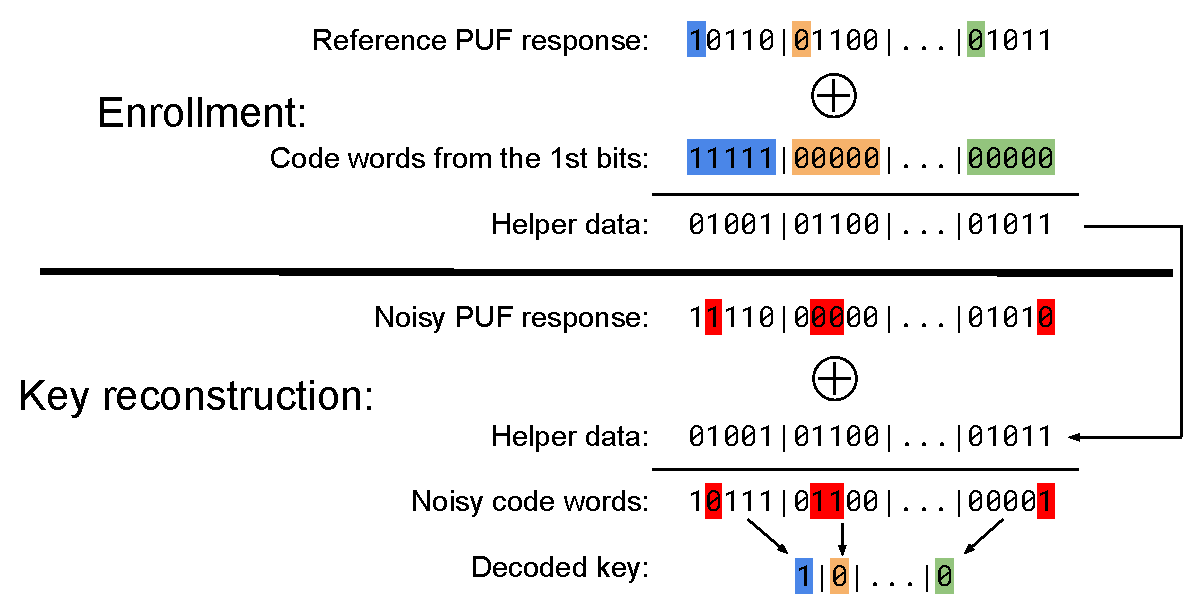
\includegraphics[width=\textwidth]{images/ecc_diagram.pdf}
    \caption[An example of enrollment and key reconstruction phases for a repetition code of length 5.]{An example of enrollment and key reconstruction phases for a repetition code of length 5. Red bits are the error bits (flipped compared to the reference response), other colors represent individual bits of the key.~\cite{Kodytek2017}}
    \label{fig:ecc_diagram}
\end{figure}

Since the \gls{ecc} can correct only a limited number of errors, the \gls{puf} response can be too noisy for the key to be properly reconstructed. The probability of this happening can be modeled using the binomial distribution. Assuming that all response bits are independent and have the same probability of error\footnote{Error is understood as a bit flip compared to the reference \gls{puf} response.}, the probability of successfully decoding a single code word can be calculated using the binomial cumulative distribution function:~\cite{Iluminada2015},~\cite{Bosch2008}

\begin{equation}\label{eq:binomial_cdf}
    F(k, n, p) = \sum_{i=0}^{k}\binom{n}{i}p^{i}(1-p^{n-i})
\end{equation}

$N$ is the size of the code word, $k$ is the maximum number of corrected errors and $p$ is the probability of a single bit error. The Equation~\ref{eq:binomial_cdf} only calculates the probability of successfully decoding a single code word which gives us only one bit of the key (because of the repetition code). To obtain the whole key, each bit is reconstructed independently and thus the probability of successful reconstruction $P_{\textrm{succ}}$ can be calculated using the Equation~\ref{eq:succ_probability}, where $B$ is the number of bits of the key (or equivalently the number of bytes of the reference response).

\begin{equation}\label{eq:succ_probability}
    P_{\textrm{succ}} = F(k, n, p)^{B} 
\end{equation}

For our case of the repetition code of length 8, maximum of three errors can be corrected in 8 bits. Therefore $n = 8$, $k = 3$ and $p$ can be estimated by the intra-Hamming distance or $1 - \textrm{reliability}$.~\cite{Iluminada2015} $B$ was chosen as $4096 \times 0.7223 \approx 2958$: a 4 KB response and 72.23~\% of stable bits (a mean value across all \glspl{mcu} using the 20~°C mask).

\cite{Bosch2008} states that key reconstruction should achieve $P_{\textrm{succ}}$ of at least $1 - 10^{-6}$ or less than one error in a million. In order to meet this requirement, the value of reliability must be greater than 99.85 \% according to the equations above. Using this knowledge, it can be concluded that a \gls{sram} \gls{puf} implementation using the 20°C stable bit mask and deep sleep power-control method is suitable only in temperatures between approximately 0 and 40 °C (see Table~\ref{table:reliability_stable_bits}). A stronger \gls{ecc} needs to be used to extend the temperature range. As the temperature range mask achieves reliability greater than 99.99 \% in all temperatures, it is suitable to be used in all tested conditions with this \gls{ecc}.

This model further calculates that $P_{\textrm{succ}}$ is 98.181 \% (or about 1 error in 55) for -40 °C and 99.913 \% (or about 1 error in 1150) for 70 °C.\footnote{Again, using the 20 °C stable bit mask and deep sleep power-control method.} However, the real-world testing showed considerably lower number of errors in key reconstructions than was predicted by this model. Results from this testing can be found in Chapter~\ref{sec:testing}

The repetition code of length eight reduces the size of the \gls{puf} response by a factor of eight. The average length of the reconstructed response thus is 2958 bits for the 20~°C stable bit mask (minimum of 2917 bits was observed for \gls{mcu} 1) and 2362 bits for the temperature range mask (minumum of 2274 bits was observed for \gls{mcu} 16). The size of the response can be doubled if 8~KB of \gls{sram} data is used instead of 4~KB. The 8~KB is however the limit for the \gls{rtc} \gls{sram} as this is the size of the memory segment used in this method.

%--------------------------------
\section{Combining power-control methods}
%--------------------------------

Two different \gls{sram} power-control methods were introduced in Chapter~\ref{sec:implementation}. The \gls{rtc} \gls{sram} method enables fast response extraction, but works reliably only in temperatures above 0°C. On the other hand, the deep sleep method is time-consuming but reliable. In this section, a design that leverages the advantages and reduces the disadvantages of the two methods is presented by combining them.

The idea is, that the \gls{rtc} \gls{sram} method will be used for temperatures it works reliably at and the deep sleep method will play a role of a fallback mechanism. For this to work, both of the methods need to reconstruct the same \gls{puf} response. The startup memory values are inherently different, as they are obtained from separate regions of memory. So to reconstruct the same \gls{puf} response every time, the generation of the \gls{ecc} helper data is altered for the \gls{rtc} \gls{sram} method.

\begin{figure}[ht!]
    \centering
    \captionsetup{justification=centering,margin=0.5cm}
    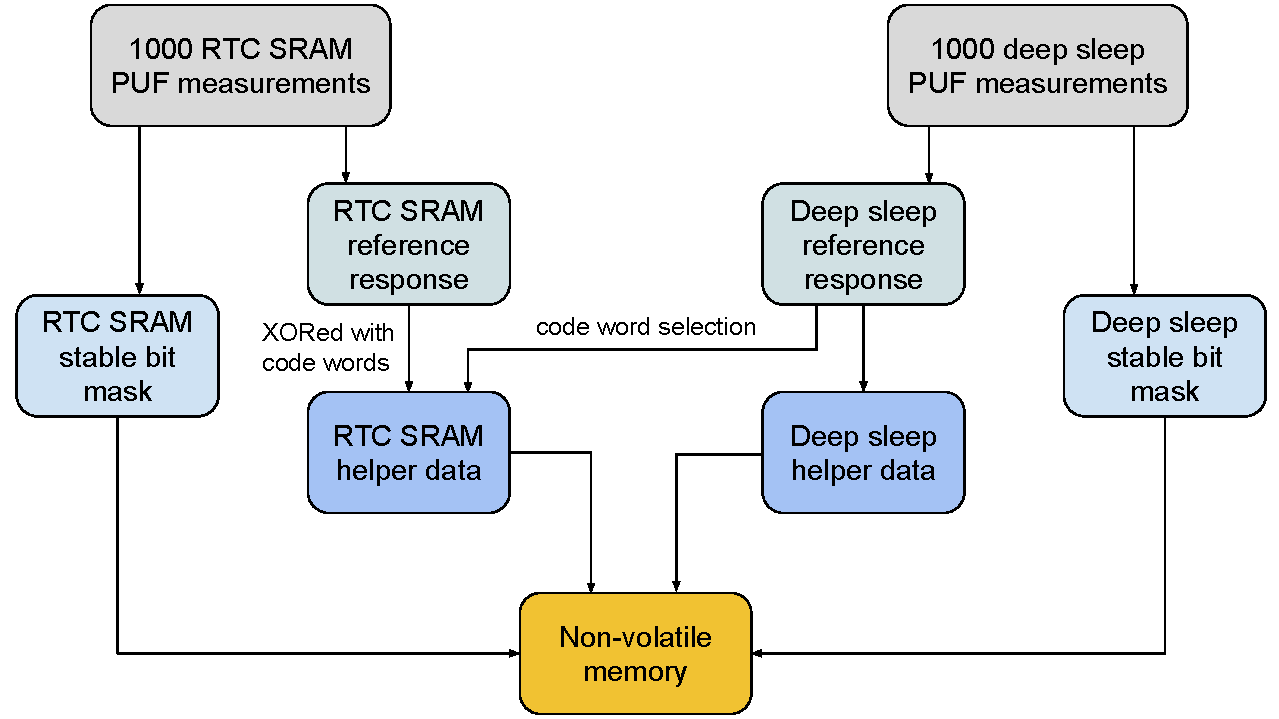
\includegraphics[width=0.85\textwidth]{images/enrollment_diagram.pdf}
    \caption{Enrollment diagram using the combination of both power-control methods to obtain the same PUF response}
    \label{fig:enrollment_diagram}
\end{figure}

\subsubsection*{Enrollment phase}

Normally, each bit of the \gls{puf} response is reconstructed from a single code word of the repetition code. This code word is determined by the first bit of the corresponding byte of the reference response. The code word is then XORed with the given byte of the reference, creating the helper data (as illustrated in Figure~\ref{fig:ecc_diagram}). So to obtain the same response after \gls{ecc} decoding, the code words for each byte of the \gls{rtc} \gls{sram} are chosen not by its reference response, but by the reference of the deep sleep method. The resulting enrollment process diagram is shown in Figure~\ref{fig:enrollment_diagram}.

\subsubsection*{Power-control method selection}

In order to choose which method to use, a detection mechanism of the freezing effect of the \gls{rtc} \gls{sram} needs to be implemented. Two indicators were chosen. The Hamming weight of the startup memory values (the memory is initialized to `0' bits before power off and about 50~\% of bits are expected to flip after power on) and the number of errors detected by the \gls{ecc}. Low Hamming weight or high error count indicate that the \gls{rtc} \gls{sram} memory froze because of low temperature and the deep sleep method needs to be used.

The mathematical model from Section~\ref{sec:ecc} tells us, that reliability needs to be at least 99.85~\%. This is equivalent to $\textrm{HD-intra} < 0.15~\%$ (or about 35 bit errors) as $\textrm{reliability = 100\% - \textrm{HD-intra}}$. Since HD-intra represents the percentage of bits that flip compared to the reference response, it can be estimated by the percentage of errors detected by the \gls{ecc}.

The Hamming weight threshold was chosen as 48.5~\%, which is lower than the uniformity values from Table~\ref{table:uniformity_rtc_sram} for non-frozen memory.

\subsubsection*{Experimental verification of the threshold values}

In order to confirm that the selected threshold values are viable and really detect the effect of memory freezing, the following experiment was conducted. Six \glspl{mcu} were continuously reconstructing their \gls{puf} responses using only the \gls{rtc} \gls{sram} method. Three data points were recorded for each reconstruction---the \gls{ecc} error detection count, the Hamming weight of the startup data and a correct reconstruction flag. The operating temperature was slowly increased from -40 to 70 °C. The resulting scatter plot can be seen in Figure~\ref{fig:correct_responses_plot}.

\begin{figure}[ht!]
    \centering
    \captionsetup{margin=0.5cm}
    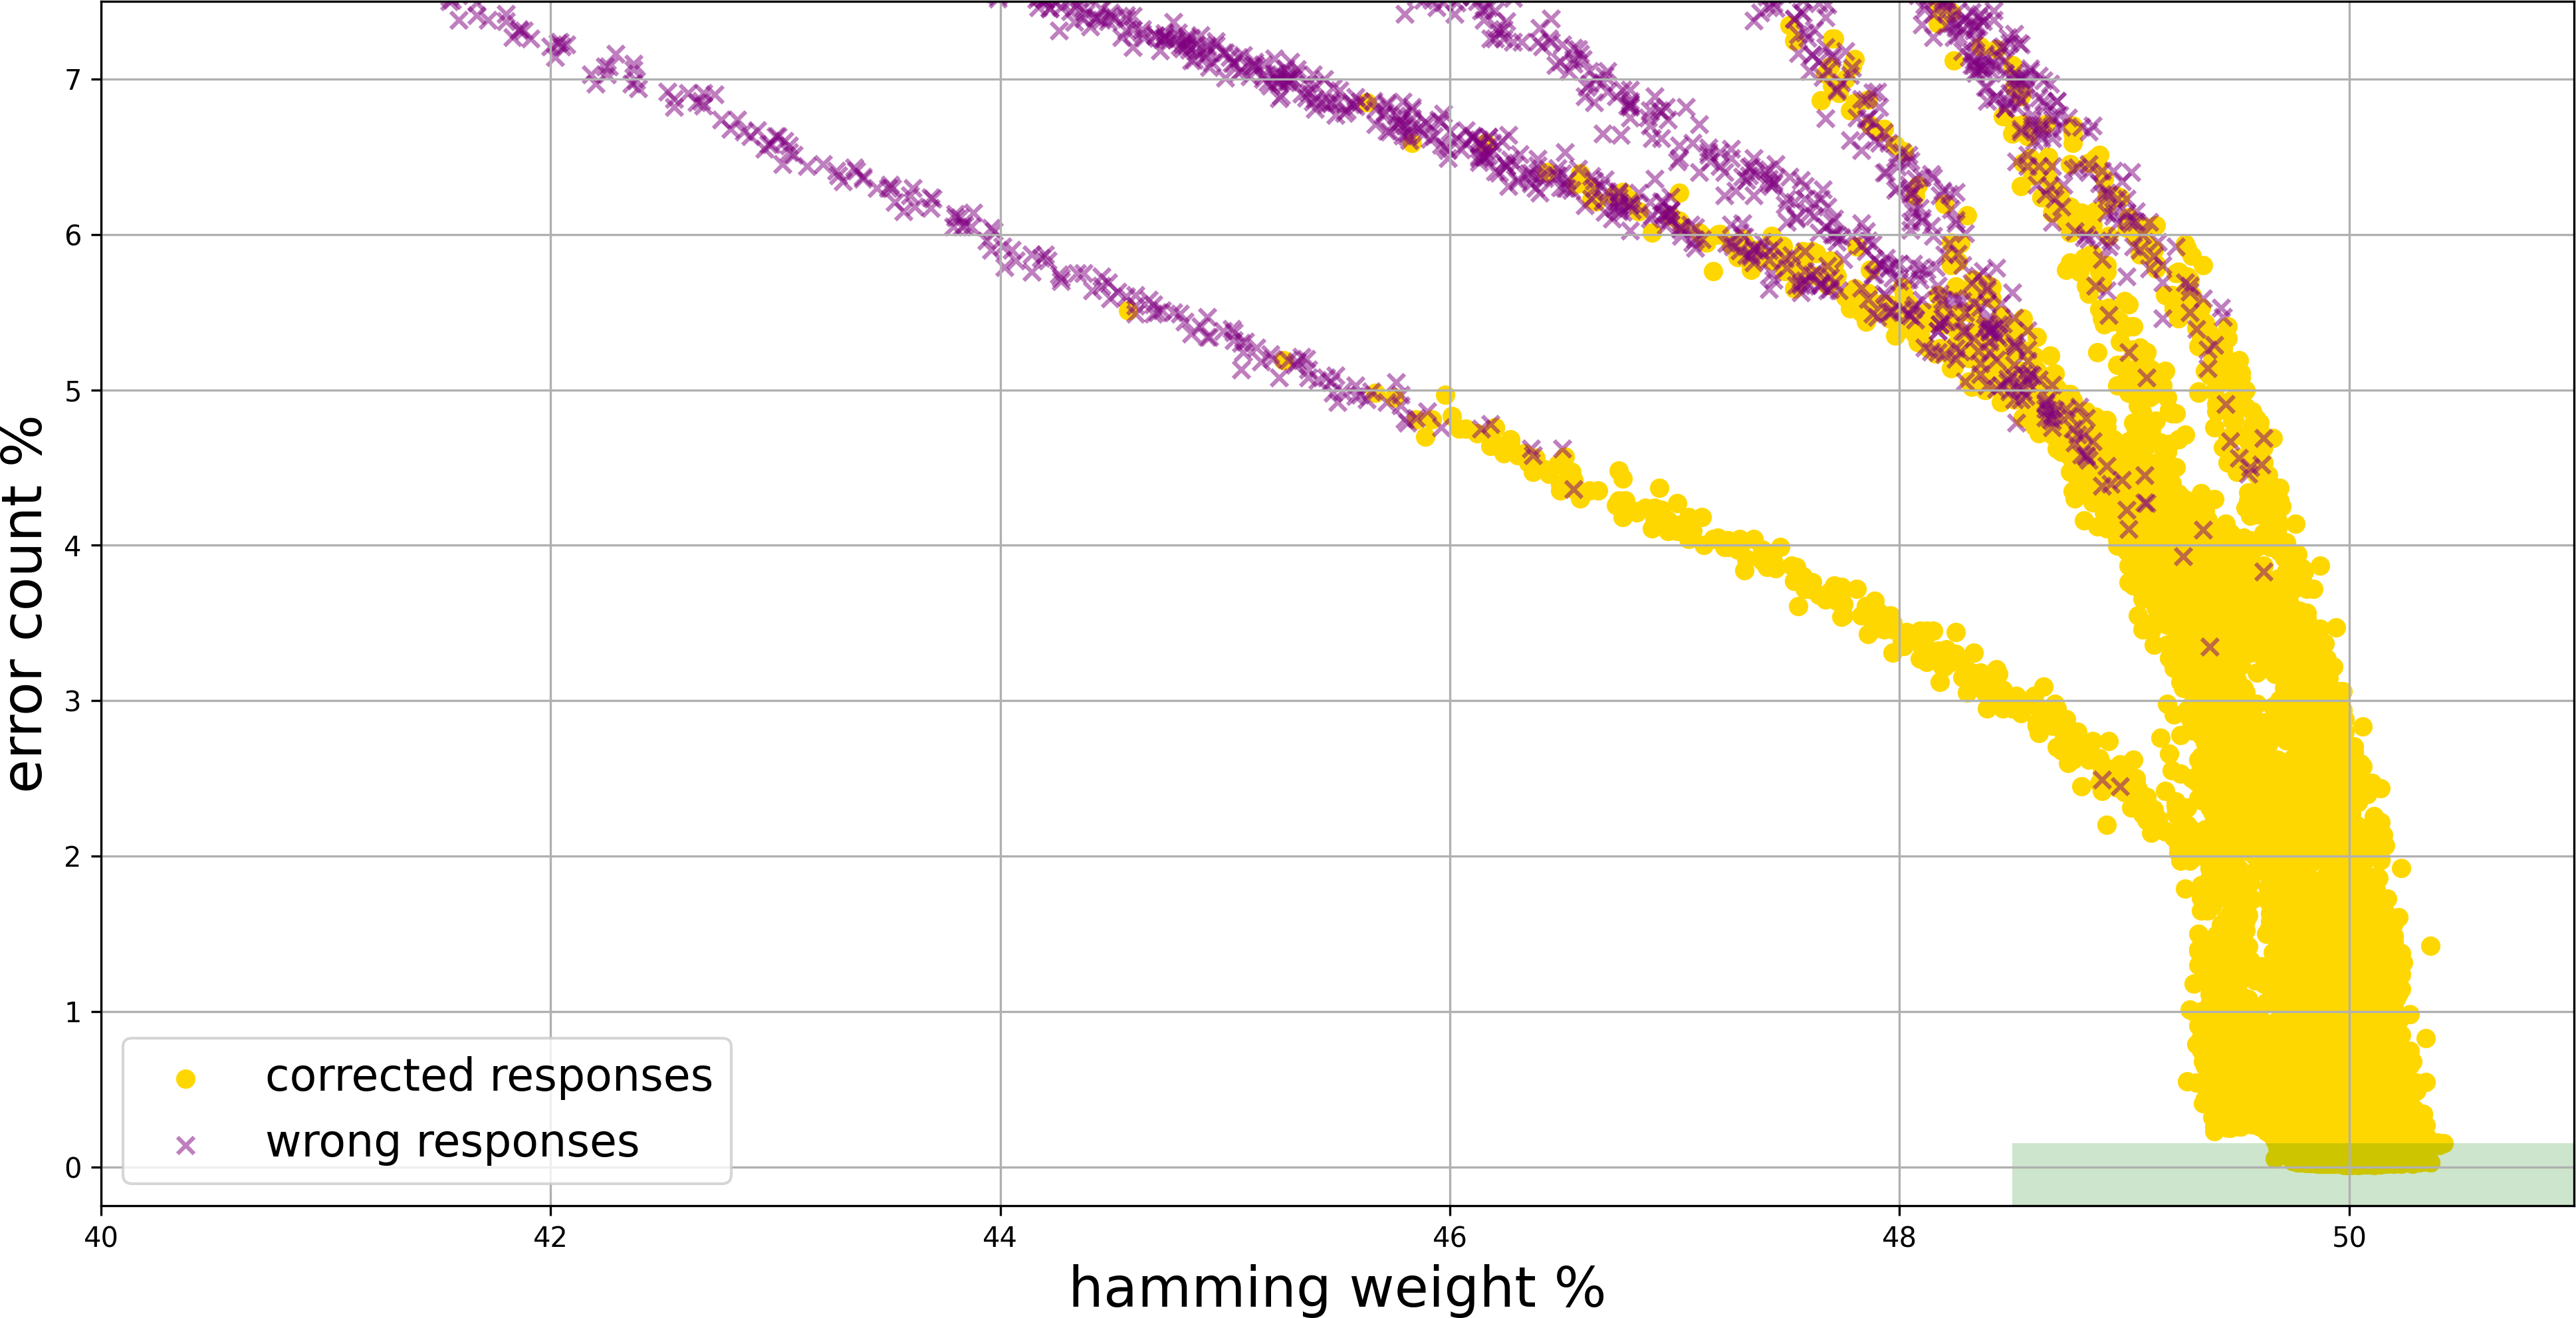
\includegraphics[width=\textwidth]{images/correct_responses_plot.png}
    \caption[A scatter plot showing the effect of Hamming weight and error count on correct response reconstruction]{A scatter plot showing the effect of Hamming weight and error count on correct response reconstruction. The green region represents data points where the \gls{rtc} \gls{sram} response is accepted as a valid response. Data obtained from \glspl{mcu} 1--6.}
    \label{fig:correct_responses_plot}
\end{figure}
% TODO caru kde beru jakoze je OK RTC SRAM metoda?

The scatter plot is zoomed-in on the part where, as the temperature increases, the responses are starting to be reconstructed properly. This happens at slightly different temperatures for each \gls{mcu}, but generally at about -5°C (the exact temperature does not matter since the threshold values do not depend on it). As expected, the error count and Hamming weight are highly negatively correlated. As the temperature increases, the Hamming weight increases and error count decreases. Once the error count is low enough (and the Hamming weight high enough), the responses can be correctly reconstructed. The lowest error rate, where the response was not reconstructed properly, is 2.45 \% (or about 580 bit errors). This proves that there is an extremely large safety margin.

\subsubsection*{Resulting design}

First, the enrollment phase is executed as is illustrated in Figure~\ref{fig:enrollment_diagram}. The resulting procedure of obtaining the \gls{puf} response is then the following:
\begin{enumerate}
    \item Try to reconstruct the \gls{puf} response using the \gls{rtc} \gls{sram} power-control method. Calculate the Hamming weight and the \gls{ecc} detected error percentage in the process.
    \item If the Hamming weight is above the threshold of 48.5~\% and the error percentage is lower than the threshold of 0.15~\%, use the reconstructed \gls{puf} response as a result and end.
    \item Reconstruct the \gls{puf} response using the deep sleep method (since the \gls{rtc} \gls{sram} method could have produced incorrect response).
\end{enumerate}

%--------------------------------
\section{Reliability testing}\label{sec:testing}
%--------------------------------

In this section, the results of testing of \gls{sram} \gls{puf} with combined power-control and reliable response reconstruction are presented. The response reconstruction process was executed 1000 times at each temperature for all \glspl{mcu}. Table~\ref{table:reconstruction_reliability} contains the percentages of successful response reconstructions using the 20 °C stable bit mask.

\begin{table}[ht!]
    \centering
    \begin{tabular}{c||rrrrrrrrrr}
    \toprule
    \textbf{MCU} & \textbf{-40°C} & \textbf{-30°C} & \textbf{-20°C} & \textbf{-10°C} & \textbf{0°C} & \textbf{10°C} & \textbf{20°C} & \textbf{30°C} & \textbf{50°C} & \textbf{70°C} \\
    \midrule
    1    &  99.9 & 100.0 & 100.0 & 100.0 & 100.0 & 100.0 & 100.0 & 100.0 & 100.0 & 100.0 \\
    2    & 100.0 & 100.0 & 100.0 & 100.0 & 100.0 & 100.0 & 100.0 & 100.0 & 100.0 & 100.0 \\
    3    &  99.9 & 100.0 & 100.0 & 100.0 & 100.0 & 100.0 & 100.0 & 100.0 & 100.0 & 100.0 \\
    4    &  98.5 & 100.0 & 100.0 & 100.0 & 100.0 & 100.0 & 100.0 & 100.0 & 100.0 & 100.0 \\
    5    & 100.0 & 100.0 & 100.0 & 100.0 & 100.0 & 100.0 & 100.0 & 100.0 & 100.0 & 100.0 \\
    6    & 100.0 & 100.0 & 100.0 & 100.0 & 100.0 & 100.0 & 100.0 & 100.0 & 100.0 & 100.0 \\
    7    & 100.0 & 100.0 & 100.0 & 100.0 & 100.0 & 100.0 & 100.0 & 100.0 & 100.0 & 100.0 \\
    8    & 100.0 & 100.0 & 100.0 & 100.0 & 100.0 & 100.0 & 100.0 & 100.0 & 100.0 & 100.0 \\
    9    & 100.0 & 100.0 & 100.0 & 100.0 & 100.0 & 100.0 & 100.0 & 100.0 & 100.0 & 100.0 \\
    10   &  98.0 & 100.0 & 100.0 & 100.0 & 100.0 & 100.0 & 100.0 & 100.0 & 100.0 & 100.0 \\
    11   &  98.8 &  99.9 & 100.0 & 100.0 & 100.0 & 100.0 & 100.0 & 100.0 & 100.0 & 100.0 \\
    12   &  99.9 & 100.0 & 100.0 & 100.0 & 100.0 & 100.0 & 100.0 & 100.0 & 100.0 & 100.0 \\
    13   & 100.0 & 100.0 & 100.0 & 100.0 & 100.0 & 100.0 & 100.0 & 100.0 & 100.0 & 100.0 \\
    14   & 100.0 & 100.0 & 100.0 & 100.0 & 100.0 & 100.0 & 100.0 & 100.0 & 100.0 & 100.0 \\
    15   &  99.9 & 100.0 & 100.0 & 100.0 & 100.0 & 100.0 & 100.0 & 100.0 & 100.0 & 100.0 \\
    16   &  99.2 & 100.0 & 100.0 & 100.0 & 100.0 & 100.0 & 100.0 & 100.0 & 100.0 &  94.7 \\
    \textbf{mean} &  99.63 &  99.99 & 100.0 & 100.0 & 100.0 & 100.0 & 100.0 & 100.0 & 100.0 &  99.67 \\
    \bottomrule
\end{tabular}
    \captionsetup{justification=centering,margin=0.5cm}
    \caption[Success rate of reliable response extraction across all MCUs and temperatures]{Success rate (\%) of reliable response extraction across all MCUs and temperatures. The 20 °C stable bit mask was used for stable bit preselection.}
    \label{table:reconstruction_reliability}
    \vspace{-1.5em}
\end{table}

The outlier in this experiment is the \gls{mcu} 16. It is the only one with incorrect reconstructions at 70~°C (and the success rate is quite low too). As this is the same \gls{mcu} as the one from Figure~\ref{fig:16_response_sleep}, lower success rate of this chip may be linked to its weird startup memory behavior.

Results using the temperature range mask are not presented, as all \glspl{mcu} reached 100 \% success rate at all temperatures. This matches expectations of the stable bits reliability results (all were above 99.99~\%).

Furthermore, the \gls{rtc} \gls{sram} method stops working at about -5~°C and 100~\% success rate was observed around this temperature. This proves that the fallback mechanism of the combined power-control \gls{puf} works reliably.

